\part*{16.09.2014 - Amplificatori Operazionali Ideali}

\section{Introduzione}

In questa sessione di laboratorio abbiamo montato due circuiti con amplificatori operazionali e valutato la loro tensione di output.

\section{Materiali}

\begin{itemize} [noitemsep]
\item Oscilloscopio Agilent DSO-X 2002A (bandwidth $70 MHz$, sample rate $2 GSa/s$);
\item Generatore di tensione continua Agilent E3631A (max $\pm 25 V$ o $\pm 6V$);
\item Generatore di tensione Agilent 33120A con range di frequenza da $100 \mu Hz$ a $15 Mhz$;
\item Multimetro Agilent 34410A (utilizzato come amperometro e per verificare i valori delle resistenze);
\item Un amplificatore operazionale UA741;
\item Resistenze di vari valori;
\item Due capacità da $0.1 \mu F$;
\item Breadboard;
\item Cablaggi vari.
\end{itemize}

\section{Premessa sugli amplificatori operazionali ideali}

Durante l'esperienza valuteremo l'amplificatore operazionale considerandolo come ideale. Infatti, in questa approssimazione (peraltro non eccessivamente limitante visti i valori di corrente in gioco nel nostro caso), valgono (considerando come A e B rispettivamente gli ingressi invertente e non invertente):

\begin{equation}
\Delta V_{AB}=0
\label{eq:regola_V}
\end{equation}
\begin{equation}
I_{AB}=0
\label{eq:regola_I}
\end{equation}

cioè la ddp fra l'ingresso invertente e non invertente è portato ad essere nullo dall'amplificatore operazionale modificando il valore di tensione in output (il cosiddetto \textit{ground virtuale} dato che nei nostri casi l'ingresso non invertente è collegato alla comune del circuito); e la corrente assorbita dall'amplificatore è nulla.
Queste regole verranno utilizzate durante questa sessione per valutare la risposta del circuito a segnali in ingresso, e si intendono utilizzate per tutte le sessioni in cui l'amplificatore è considerato ideale.

\begin{figure}[ht]
 \centering
   {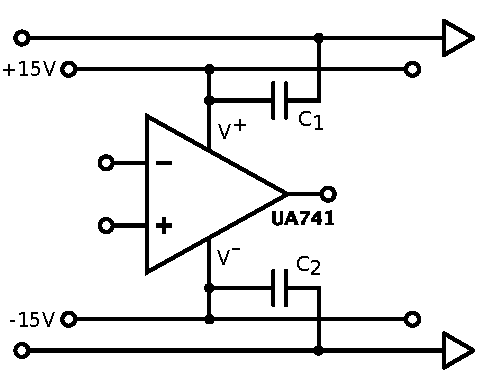
\includegraphics[width=6cm]{alimentazione.pdf}}
 \caption{Grafico dell'alimentazione dell'OPAMP. La tensione di alimentazione è fornita con il generatore di tensione costante, mentre le capacità sono $C_1=C_2=0.1 \mu F$. Per maggiore chiarezza negli schemi circuitali, questa configurazione sarà nascosta negli schemi successivi, ma comunque presente sulla breadboard.}
 \label{gr:costante}
\end{figure}

Inoltre, per maggiore chiarezza degli schemi circuitali, l'amplificatore si intende collegato all'alimentazione ($\pm 15 V$); e, al fine di evitare problemi di noise durante l'alimentazione, abbiamo collegato l'alimentazione a due capacità come nello schema.

\section{Generatore di corrente}

In questo circuito montiamo un generatore di corrente costante, cioè un dispositivo in grado di erogare una corrente costante indipendentemente dal carico a cui è sottoposto. Per valutare la risposta a diverse resistenze di carico abbiamo dunque utilizzato come $R_f$ una resistenza variabile di tipo \textit{trimmer}. Lo schema circuitale è in figura.

\begin{wrapfigure}[21]{r}{0.55\textwidth}
  \begin{center}
    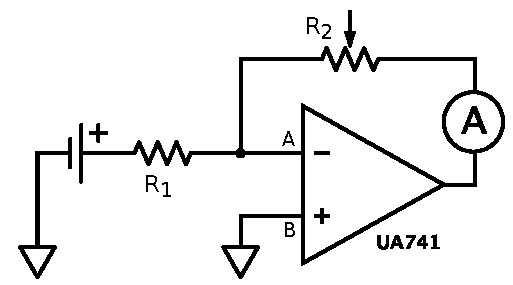
\includegraphics[width=0.40\textwidth]{c1.pdf}
  \end{center}
  \caption{Schema del generatore di corrente costante. Come valori abbiamo utilizzato $R1=3.85 \pm 0.01 k\Omega$ e $V_{gen}=3.85 V$, mentre $R_2$ è variabile. Come amperometro è utilizzato il multimetro, mentre per alimentare l'OPAMP e come generatore di tensione costante in figura, abbiamo utillizzato il generatore di tensione continua.}
\end{wrapfigure}

Risolviamo ora il circuito. Dato che B si trova a potenziale di comune, per (\ref{eq:regola_V}) anche A sarà allo stesso potenziale, che considereremo nullo. Dunque varrà
\begin{equation}
V_{gen}=I R_1
\label{eq:gen_1}
\end{equation}
Per (\ref{eq:regola_I}) e la legge di Kirkhhoff sui nodi, avremo invece che la corrente passante per la resistenza di carico è uguale alla corrente $I$ di (\ref{eq:gen_1}).

Otteniamo dunque che la tensione di output si modificherà, ad opera dell'OPAMP, in modo da far passare sempre lo stesso valore di corrente attraverso $R_2$; ciò avviene per il fenomeno di retroazione negativa, che ci permette di controllare la tensione di output tramite la resistenza di feedback, che in questo caso è proprio $R_2$, e di ottenere dunque una corrente costante passante per il circuito di feedback. Imponendo l'uguaglianza della corrente possiamo inoltre trovare il valore della tensione di uscita
$$V_{out}=\frac{R_2}{R_1} V_{gen}$$

Durante l'esperienza abbiamo però deciso di misurare la corrente passante per la resistenza piuttosto che la tensione di uscita, ponendo un amperometro fra l'uscita dell'OPAMP e la resistenza di carico $R_2$. Come valore di corrente abbiamo scelto $1 mA$ in modo da discostarci dalla corrente massima in cui l'amplificatore operazionale potrebbe non comportarsi più in maniera ideale ($10/20 mA$); e avendo a disposizione una resistenza $R_1=3.85 \pm 0.01 k\Omega$, per (\ref{eq:gen_1}), abbiamo utilizzato una tensione continua di $3.85 V$. Di seguito proponiamo alcuni valori sperimentali che confermano la capacità del circuito da noi creato di fornire alla resistenza di carico una corrente costante di $1 mA$ (considerando gli errori sull'ultima cifra come unitari).

\begin{center}
\begin{tabular}{c|c|c|c|c|c|c|c|c}
Resistenza variabile [$\Omega$] & 0.54 & 35.1 & 412 & 1021 & 1996 & 3068 & 4170 & 4719 \\ 
\hline 
Corrente nel carico [$mA$] & 1.002 & 1.002 & 1.002 & 1.002 & 1.002 & 1.002 & 1.002 & 1.002 \\ 
\end{tabular}
\end{center}

\section{Sommatore Pesato}

Valutiamo ora il sommatore pesato, cioè un circuito che dati due segnali in ingresso li somma con relativi pesi dati dal rapporto fra la resistenza di feedback ($R_f$) e quella a loro associata ($R_1$ e $R_2$). Lo schema circuitale è in figura.

\begin{wrapfigure}[21]{l}{0.55\textwidth}
  \begin{center}
    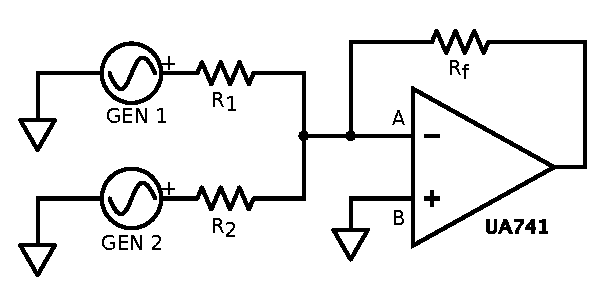
\includegraphics[width=0.40\textwidth]{c2.pdf}
  \end{center}
  \caption{Schema del sommatore pesato. Come valori abbiamo utilizzato $R_f \approx R_1=(99.9 \pm 0.1) k \Omega$ e $R_2=(49.8 \pm 0.1) k \Omega$, dove per $R_2$ è stato necessario utilizzare un parallelo di due resistenza da $100 k\Omega$. Come GEN 1 abbiamo utilizzato l'oscilloscopio, mentre per GEN 2 il generatore di forme d'onda. Infine, per valutare la tensione in uscita abbiamo utilizzato l'oscilloscopio.}
\end{wrapfigure}

Per risolvere il circuito consideriamo, definendo le tensioni dei generatori 1 e 2 rispettivamente $V_1$ e $V_2$, le seguenti equazioni derivanti dalle leggi di Kirkhhoff e dalla (\ref{eq:regola_I})
$$V_1 - V_A =I_1 R_1 \qquad V_2 - V_A =I_2 R_2$$
$$V_A - V_{out} =(I_1+I_2) R_f$$
Per (\ref{eq:regola_V}) vale inoltre che $V_A=V_B=0$; dunque otteniamo, sostituendo le correnti nell'ultima equazione sopra
$$V_{out}=-R_f \left( \frac{V_1}{R_1}+\frac{V_2}{R_2}\right)$$

Si potrebbe dunque definire un peso relativo $\phi_i$ ad ogni segnale dato dal rapporto fra $R_f$ ed $R_{i}$ (con $i=1,2$) e scrivere una formula del tipo
$$V_{out}=-\sum^{2}_{i=1} \frac{R_f}{R_{i}}V_{i}=-\sum^{2}_{i=1} \phi_i V_{i}$$

Durante l'esperienza abbiamo optato per valori semplici dei rapporti fra le resistenze. Abbiamo dunque utilizzato i seguenti valori di resistenza: $R_f=R_1=100 k\Omega$ e $R_2=50 k\Omega$; si ottengono dunque $\phi_1=1$ e $\phi_2=2$.

Presentiamo ora i grafici di alcune forme d'onda in uscita.

\begin{figure}[ht]
 \centering
   {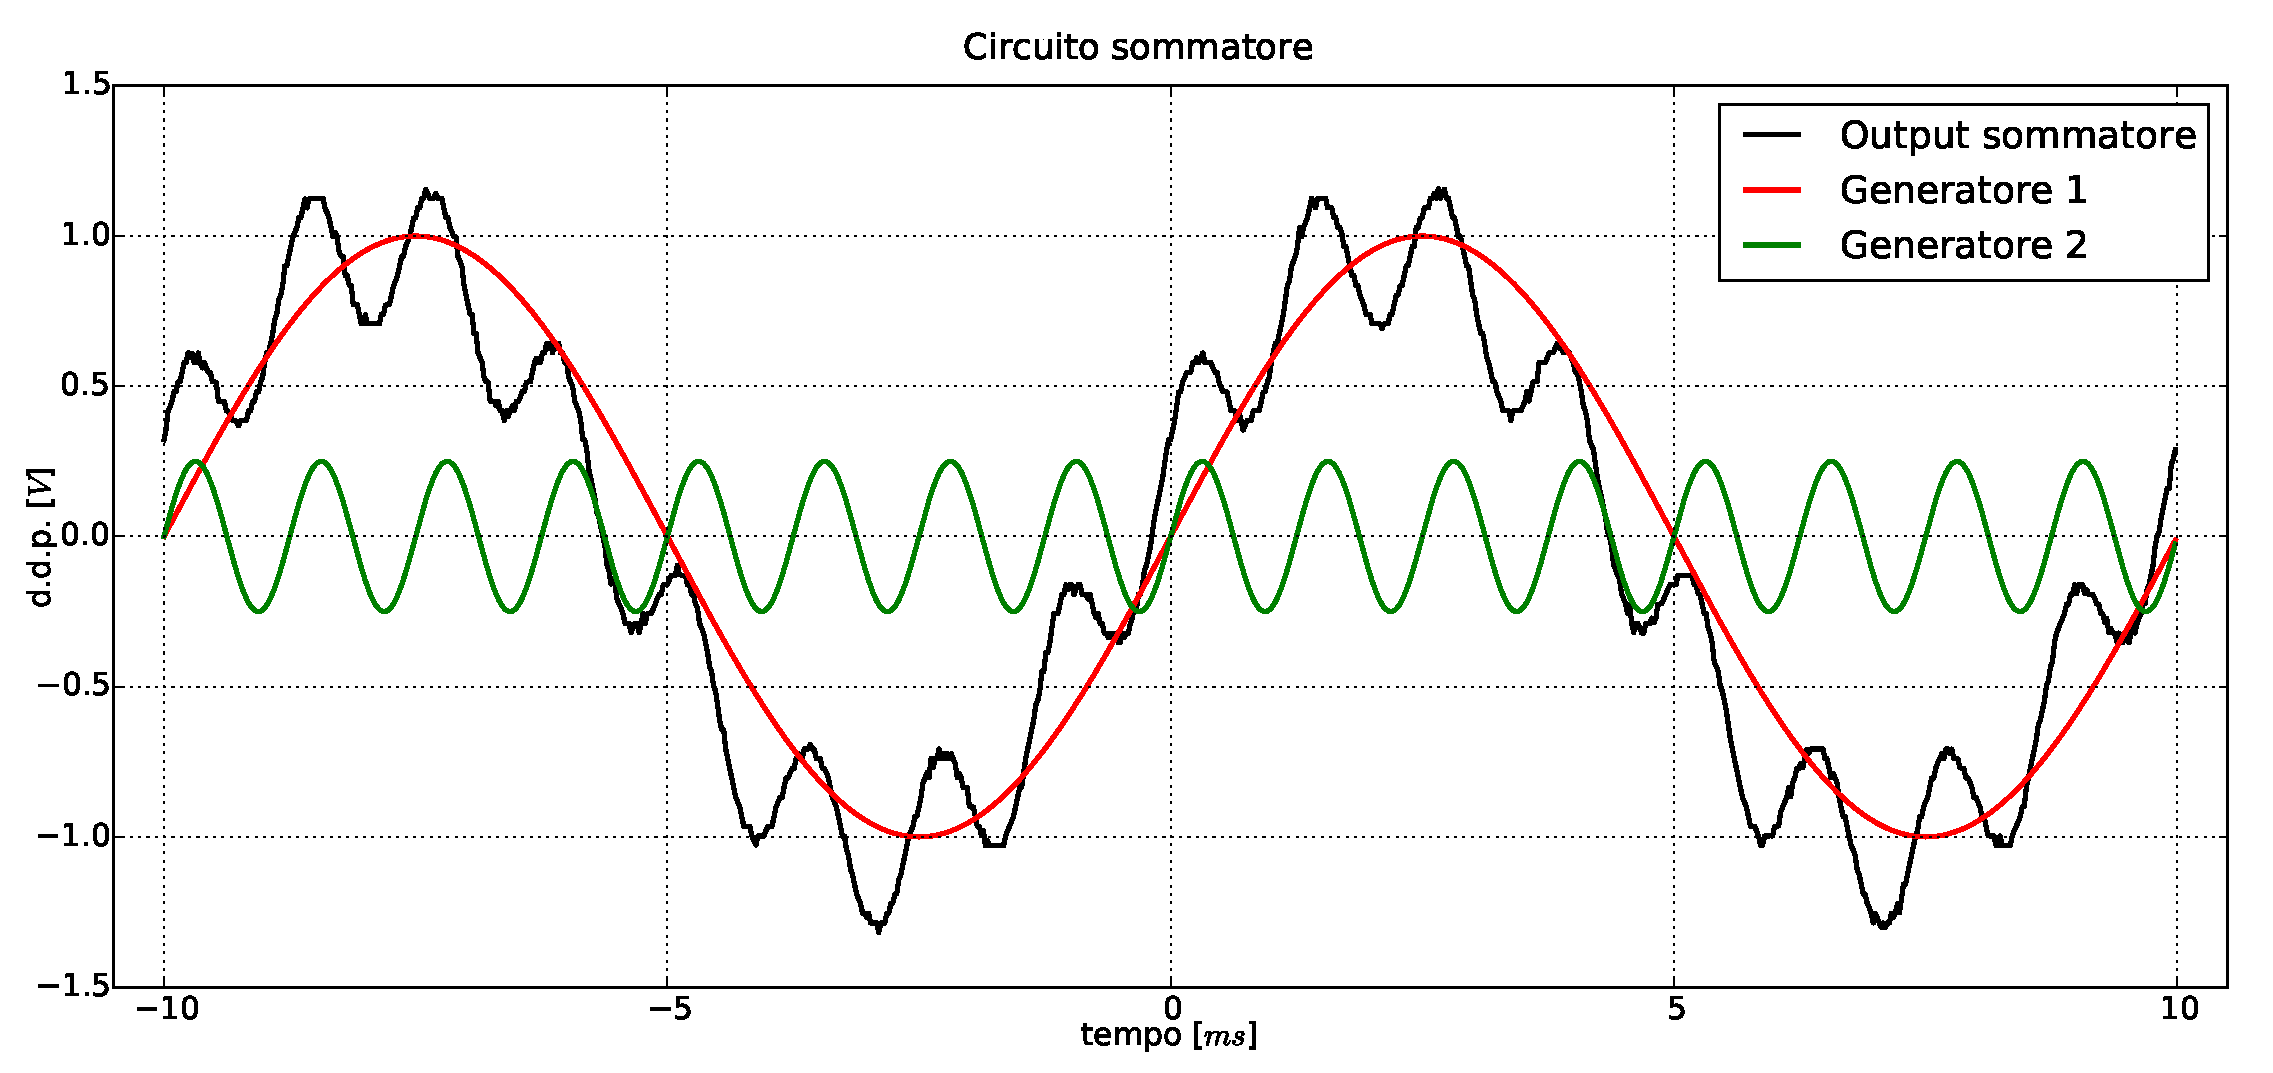
\includegraphics[width=18cm]{sinsin.pdf}}
 \caption{Grafico della tensione di uscita. Il generatore 1 (generatore dell'oscilloscopio) crea un'onda sinusoidale di $\nu=800 Hz$ e $V^1_{pp}=250 mV$; il generatore 2 (generatore di forme d'onda) crea invece un'onda sinusoidale di $\nu=100 Hz$ e $V^2_{pp}=500 mV$. Notiamo inoltre che l'ampiezza massima è pari a $\phi_1 V^1_{pp}+\phi_2 V^2_{pp}=1250 mV$.}
 \label{gr:costante}
\end{figure}

\begin{figure}[ht]
 \centering
   {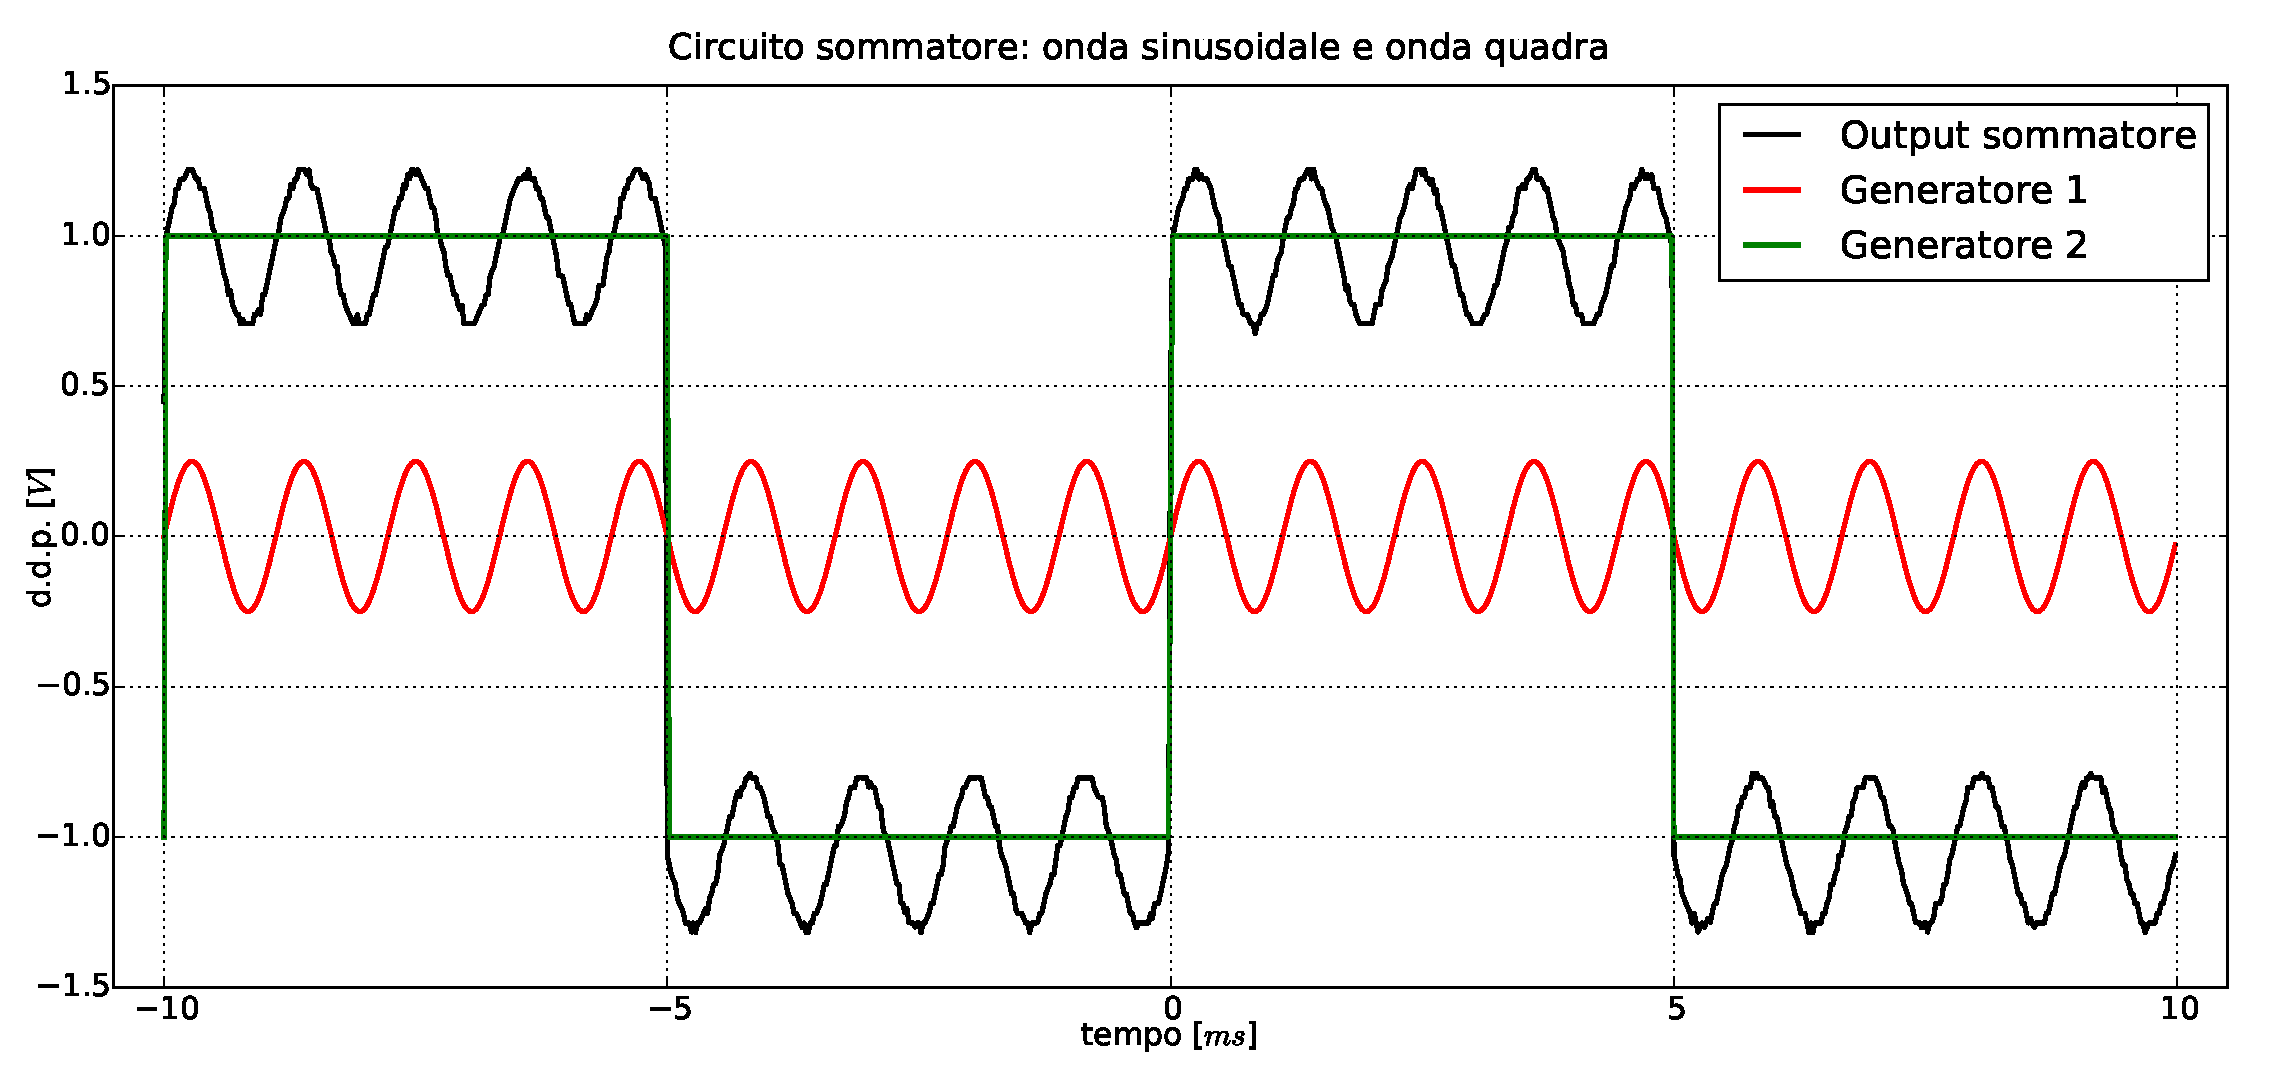
\includegraphics[width=18cm]{sinquad.pdf}}
 \caption{Grafico della tensione di uscita. Il generatore 1 (generatore dell'oscilloscopio) crea un'onda sinusoidale di $\nu=900 Hz$ e $V^1_{pp}=250 mV$; il generatore 2 (generatore di forme d'onda) crea invece un'onda quadra di $\nu=100 Hz$ e $V^2_{pp}=500 mV$. Notiamo inoltre che anche in questo caso l'ampiezza massima è pari a $\phi_1 V^1_{pp}+\phi_2 V^2_{pp}=1250 mV$.}
 \label{gr:costante}
\end{figure}